\documentclass[10pt]{article}
\usepackage[polish]{babel}
\usepackage[utf8]{inputenc}
\usepackage[T1]{fontenc}
\usepackage{graphicx}
\usepackage[export]{adjustbox}
\graphicspath{ {./images/} }
\usepackage{amsmath}
\usepackage{amsfonts}
\usepackage{amssymb}
\usepackage[version=4]{mhchem}
\usepackage{stmaryrd}
\usepackage{multirow}

\title{EGZAMIN MATURALNY Z MATEMATYKI \\
 POZIOM ROZSZERZONY }

\author{}
\date{}


\begin{document}
\maketitle

\includegraphics[max width=\textwidth, center]{2024_11_21_606d6e4e152fe3e9f6feg-01}\\
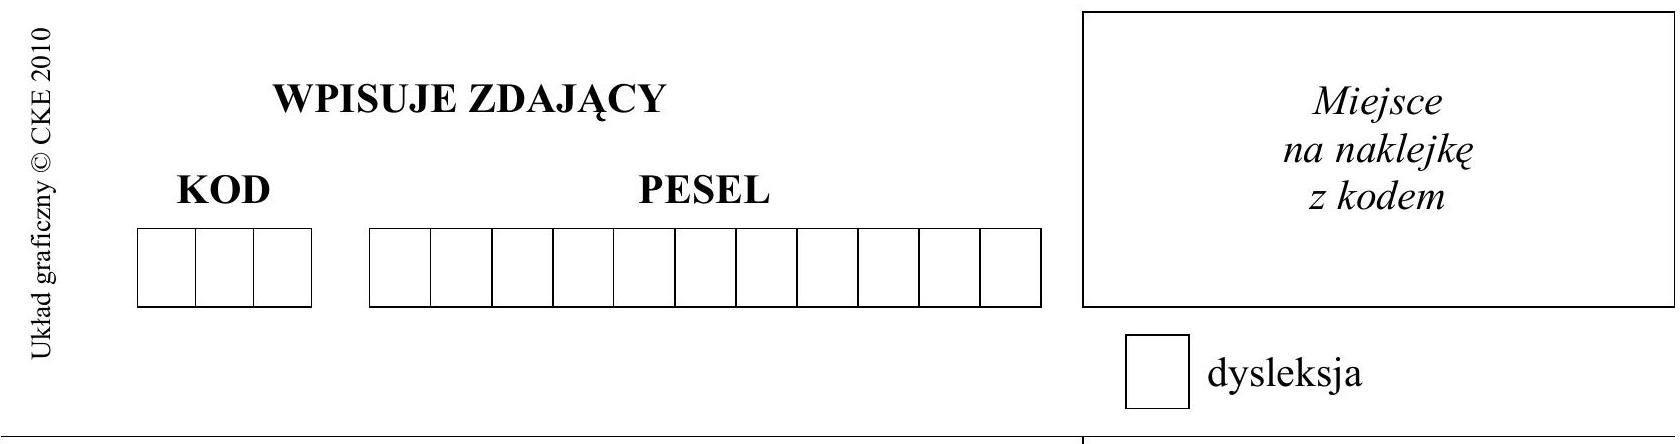
\includegraphics[max width=\textwidth, center]{2024_11_21_606d6e4e152fe3e9f6feg-01(1)}

MAJ 2012

\begin{enumerate}
  \item Sprawdź, czy arkusz egzaminacyjny zawiera 19 stron (zadania \(1-11\) ). Ewentualny brak zgłoś
\end{enumerate}

Czas pracy: 180 minut

Liczba punktów do uzyskania: 50

MMA-R1\_1P-122

\section*{Zadanie 1. (4 pkt)}
Wyznacz cztery kolejne liczby całkowite takie, że największa z nich jest równa sumie kwadratów trzech pozostałych liczb.\\

\includegraphics[max width=\textwidth, center]{2024_11_21_606d6e4e152fe3e9f6feg-02}\\

\includegraphics[max width=\textwidth, center]{2024_11_21_606d6e4e152fe3e9f6feg-03}

Odpowiedź:

\begin{center}
\begin{tabular}{|c|l|c|}
\hline
\multirow{2}{*}{\begin{tabular}{l}
Wypetnia \\
egzaminator \\
\end{tabular}} & Nr zadania & 1. \\
\cline { 2 - 3 }
 & Maks. liczba pkt & 4 \\
\cline { 2 - 3 }
 & Uzyskana liczba pkt &  \\
\hline
\end{tabular}
\end{center}

\section*{Zadanie 2. (4 pkt)}
Rozwiąż nierówność \(x^{4}+x^{2} \geq 2 x\).\\

\includegraphics[max width=\textwidth, center]{2024_11_21_606d6e4e152fe3e9f6feg-04}

Odpowiedź:

\section*{Zadanie 3. (4 pkt)}
Rozwiąż równanie \(\cos 2 x+2=3 \cos x\).\\

\includegraphics[max width=\textwidth, center]{2024_11_21_606d6e4e152fe3e9f6feg-05}

Odpowiedź:

\begin{center}
\begin{tabular}{|c|l|c|c|}
\hline
\multirow{2}{*}{\begin{tabular}{c}
Wypełnia \\
egzaminator \\
\end{tabular}} & Nr zadania & 2. & 3. \\
\cline { 2 - 4 }
 & Maks. liczba pkt & \(\mathbf{4}\) & \(\mathbf{4}\) \\
\cline { 2 - 4 }
 & Uzyskana liczba pkt &  &  \\
\hline
\end{tabular}
\end{center}

\section*{Zadanie 4. (6 pkt)}
Oblicz wszystkie wartości parametru \(m\), dla których równanie \(x^{2}-(m+2) x+m+4=0\) ma dwa różne pierwiastki rzeczywiste \(x_{1}, x_{2}\) takie, że \(x_{1}^{4}+x_{2}^{4}=4 m^{3}+6 m^{2}-32 m+12\).\\

\includegraphics[max width=\textwidth, center]{2024_11_21_606d6e4e152fe3e9f6feg-06}\\

\includegraphics[max width=\textwidth, center]{2024_11_21_606d6e4e152fe3e9f6feg-07}

Odpowiedź:

\begin{center}
\begin{tabular}{|c|l|c|}
\hline
\multirow{2}{*}{\begin{tabular}{l}
Wypetnia \\
egzaminator \\
\end{tabular}} & Nr zadania & 4. \\
\cline { 2 - 3 }
 & Maks. liczba pkt & 6 \\
\cline { 2 - 3 }
 & Uzyskana liczba pkt &  \\
\hline
\end{tabular}
\end{center}

\section*{Zadanie 5. (6 pkt)}
Trzy liczby tworzą ciąg geometryczny. Jeżeli do drugiej liczby dodamy 8 , to ciąg ten zmieni się w arytmetyczny. Jeżeli zaś do ostatniej liczby nowego ciągu arytmetycznego dodamy 64, to tak otrzymany ciag będzie znów geometryczny. Znajdź te liczby. Uwzględnij wszystkie możliwości.\\

\includegraphics[max width=\textwidth, center]{2024_11_21_606d6e4e152fe3e9f6feg-08}\\

\includegraphics[max width=\textwidth, center]{2024_11_21_606d6e4e152fe3e9f6feg-09}

Odpowiedź:

\begin{center}
\begin{tabular}{|c|l|c|}
\hline
\multirow{2}{*}{\begin{tabular}{l}
Wypetnia \\
egzaminator \\
\end{tabular}} & Nr zadania & 5. \\
\cline { 2 - 3 }
 & Maks. liczba pkt & \(\mathbf{6}\) \\
\cline { 2 - 3 }
 & Uzyskana liczba pkt &  \\
\hline
\end{tabular}
\end{center}

\section*{Zadanie 6. (6 pkt)}
W układzie współrzędnych rozważmy wszystkie punkty \(P\) postaci: \(P=\left(\frac{1}{2} m+\frac{5}{2}, m\right)\), gdzie \(m \in\langle-1,7\rangle\). Oblicz najmniejszą i największą wartość \(|P Q|^{2}\), gdzie \(Q=\left(\frac{55}{2}, 0\right)\).

\begin{center}
\begin{tabular}{|c|c|c|c|c|c|c|c|c|c|c|c|c|c|c|c|c|c|c|c|c|c|c|}
\hline
 &  &  &  &  &  &  &  &  &  &  &  &  &  &  &  &  &  &  &  &  &  &  \\
\hline
 &  &  &  &  &  &  &  &  &  &  &  &  &  &  &  &  &  &  &  &  &  &  \\
\hline
 &  &  &  &  &  &  &  &  &  &  &  &  &  &  &  &  &  &  &  &  &  &  \\
\hline
 &  &  &  &  &  &  &  &  &  &  &  &  &  &  &  &  &  &  &  &  &  &  \\
\hline
 &  &  &  &  &  &  &  &  &  &  &  &  &  &  &  &  &  &  &  &  &  &  \\
\hline
 &  &  &  &  &  &  &  &  &  &  &  &  &  &  &  &  &  &  &  &  &  &  \\
\hline
 &  &  &  &  &  &  &  &  &  &  &  &  &  &  &  &  &  &  &  &  &  &  \\
\hline
 &  &  &  &  &  &  &  &  &  &  &  &  &  &  &  &  &  &  &  &  &  &  \\
\hline
 &  &  &  &  &  &  &  &  &  &  &  &  &  &  &  &  &  &  &  &  &  &  \\
\hline
 &  &  &  &  &  &  &  &  &  &  &  &  &  &  &  &  &  &  &  &  &  &  \\
\hline
 &  &  &  &  &  &  &  &  &  &  &  &  &  &  &  &  &  &  &  &  &  &  \\
\hline
 &  &  &  &  &  &  &  &  &  &  &  &  &  &  &  &  &  &  &  &  &  &  \\
\hline
 &  &  &  &  &  &  &  &  &  &  &  &  &  &  &  &  &  &  &  &  &  &  \\
\hline
 &  &  &  &  &  &  &  &  &  &  &  &  &  &  &  &  &  &  &  &  &  &  \\
\hline
 &  &  &  &  &  &  &  &  &  &  &  &  &  &  &  &  &  &  &  &  &  &  \\
\hline
 &  &  &  &  &  &  &  &  &  &  &  &  &  &  &  &  &  &  &  &  &  &  \\
\hline
 &  &  &  &  &  &  &  &  &  &  &  &  &  &  &  &  &  &  &  &  &  &  \\
\hline
 &  &  &  &  &  &  &  &  &  &  &  &  &  &  &  &  &  &  &  &  &  &  \\
\hline
 &  &  &  &  &  &  &  &  &  &  &  &  &  &  &  &  &  &  &  &  &  &  \\
\hline
 &  &  &  &  &  &  &  &  &  &  &  &  &  &  &  &  &  &  &  &  &  &  \\
\hline
 &  &  &  &  &  &  &  &  &  &  &  &  &  &  &  &  &  &  &  &  &  &  \\
\hline
 &  &  &  &  &  &  &  &  &  &  &  &  &  &  &  &  &  &  &  &  &  &  \\
\hline
 &  &  &  &  &  &  &  &  &  &  &  &  &  &  &  &  &  &  &  &  &  &  \\
\hline
 &  &  &  &  &  &  &  &  &  &  &  &  &  &  &  &  &  &  &  &  &  &  \\
\hline
 &  &  &  &  &  &  &  &  &  &  &  &  &  &  &  &  &  &  &  &  &  &  \\
\hline
 &  &  &  &  &  &  &  &  &  &  &  &  &  &  &  &  &  &  &  &  &  &  \\
\hline
 &  &  &  &  &  &  &  &  &  &  &  &  &  &  &  &  &  &  &  &  &  &  \\
\hline
 &  &  &  &  &  &  &  &  &  &  &  &  &  &  &  &  &  &  &  &  &  &  \\
\hline
 &  &  &  &  &  &  &  &  &  &  &  &  &  &  &  &  &  &  &  &  &  &  \\
\hline
 &  &  &  &  &  &  &  &  &  &  &  &  &  &  &  &  &  &  &  &  &  &  \\
\hline
 &  &  &  &  &  &  &  &  &  &  &  &  &  &  &  &  &  &  &  &  &  &  \\
\hline
 &  &  &  &  &  &  &  &  &  &  &  &  &  &  &  &  &  &  &  &  &  &  \\
\hline
 &  &  &  &  &  &  &  &  &  &  &  &  &  &  &  &  &  &  &  &  &  &  \\
\hline
 &  &  &  &  &  &  &  &  &  &  &  &  &  &  &  &  &  &  &  &  &  &  \\
\hline
 &  &  &  &  &  &  &  &  &  &  &  &  &  &  &  &  &  &  &  &  &  &  \\
\hline
 &  &  &  &  &  &  &  &  &  &  &  &  &  &  &  &  &  &  &  &  &  &  \\
\hline
 &  &  &  &  &  &  &  &  &  &  &  &  &  &  &  &  &  &  &  &  &  &  \\
\hline
 &  &  &  &  &  &  &  &  &  &  &  &  &  &  &  &  &  &  &  &  &  &  \\
\hline
 &  &  &  &  &  &  &  &  &  &  &  &  &  &  &  &  &  &  &  &  &  &  \\
\hline
 &  &  &  &  &  &  &  &  &  &  &  &  &  &  &  &  &  &  &  &  &  &  \\
\hline
 &  &  &  &  &  &  &  &  &  &  &  &  &  &  &  &  &  &  &  &  &  &  \\
\hline
 &  &  &  &  &  &  &  &  &  &  &  &  &  &  &  &  &  &  &  &  &  &  \\
\hline
 &  &  &  &  &  &  &  &  &  &  &  &  &  &  &  &  &  &  &  &  &  &  \\
\hline
 &  &  &  &  &  &  &  &  &  &  &  &  &  &  &  &  &  &  &  &  &  &  \\
\hline
\end{tabular}
\end{center}

\begin{center}

\includegraphics[max width=\textwidth]{2024_11_21_606d6e4e152fe3e9f6feg-11}
\end{center}

Odpowiedź:

\begin{center}
\begin{tabular}{|c|l|c|}
\hline
\multirow{2}{*}{\begin{tabular}{l}
Wypelnia \\
egzaminator \\
\end{tabular}} & Nr zadania & \(\mathbf{6 .}\) \\
\cline { 2 - 3 }
 & Maks. liczba pkt & \(\mathbf{6}\) \\
\cline { 2 - 3 }
 & Uzyskana liczba pkt &  \\
\hline
\end{tabular}
\end{center}

\section*{Zadanie 7. (3 pkt)}
Udowodnij, że jeżeli \(a+b \geq 0\), to prawdziwa jest nierówność \(a^{3}+b^{3} \geq a^{2} b+a b^{2}\).\\

\includegraphics[max width=\textwidth, center]{2024_11_21_606d6e4e152fe3e9f6feg-12}

Zadanie 8. (4 pht)\\
Oblicz, ile jest liczb naturalnych ośmiocyfrowych takich, że iloczyn cyfr w ich zapisie dziesiętnym jest równy 12.\\

\includegraphics[max width=\textwidth, center]{2024_11_21_606d6e4e152fe3e9f6feg-13}

Odpowiedź:

\begin{center}
\begin{tabular}{|c|l|c|c|}
\hline
\multirow{2}{*}{\begin{tabular}{c}
Wypelnia \\
egzaminator \\
\end{tabular}} & Nr zadania & \(\mathbf{7 .}\) & \(\mathbf{8 .}\) \\
\cline { 2 - 4 }
 & Maks. liczaba pkt & \(\mathbf{3}\) & \(\mathbf{4}\) \\
\cline { 2 - 4 }
 & Uzyskana liczba pkt &  &  \\
\hline
\end{tabular}
\end{center}

\section*{Zadanie 9. (5 pkt)}
Dany jest prostokąt \(A B C D\), w którym \(|A B|=a,|B C|=b\) i \(a>b\). Odcinek \(A E\) jest wysokością trójkąta \(D A B\) opuszczoną na jego bok \(B D\). Wyraź pole trójkąta \(A E D\) za pomocą \(a\) i \(b\).\\

\includegraphics[max width=\textwidth, center]{2024_11_21_606d6e4e152fe3e9f6feg-14}\\

\includegraphics[max width=\textwidth, center]{2024_11_21_606d6e4e152fe3e9f6feg-15}

Odpowiedź:

\begin{center}
\begin{tabular}{|c|l|c|}
\hline
\multirow{2}{*}{\begin{tabular}{l}
Wypelnia \\
egzaminator \\
\end{tabular}} & Nr zadania & 9. \\
\cline { 2 - 3 }
 & Maks. liczba pkt & 5 \\
\cline { 2 - 3 }
 & Uzyskana liczba pkt &  \\
\hline
\end{tabular}
\end{center}

Zadanie 10. (5 pkt)\\
Podstawą ostrosłupa \(A B C S\) jest trójkąt równoramienny \(A B C\). Krawędź \(A S\) jest wysokością ostrosłupa oraz \(|A S|=8 \sqrt{210},|B S|=118,|C S|=131\). Oblicz objętość tego ostrosłupa.\\

\includegraphics[max width=\textwidth, center]{2024_11_21_606d6e4e152fe3e9f6feg-16}\\

\includegraphics[max width=\textwidth, center]{2024_11_21_606d6e4e152fe3e9f6feg-17}

Odpowiedź:

\begin{center}
\begin{tabular}{|c|l|c|}
\hline
\multirow{2}{*}{\begin{tabular}{l}
Wypetnia \\
egzaminator \\
\end{tabular}} & Nr zadania & 10. \\
\cline { 2 - 3 }
 & Maks. liczba pkt & 5 \\
\cline { 2 - 3 }
 & Uzyskana liczba pkt &  \\
\hline
\end{tabular}
\end{center}

\section*{Zadanie 11. (3 pkt)}
Zdarzenia losowe \(A, B\) są zawarte w \(\Omega\) oraz \(P\left(A \cap B^{\prime}\right)=0,7\) ( \(A^{\prime}\) oznacza zdarzenie przeciwne do zdarzenia \(A, B^{\prime}\) oznacza zdarzenie przeciwne do zdarzenia \(B\) ).\\
Wykaż, że \(P\left(A^{\prime} \cap B\right) \leq 0,3\).\\

\includegraphics[max width=\textwidth, center]{2024_11_21_606d6e4e152fe3e9f6feg-18}

\begin{center}
\begin{tabular}{|c|l|c|}
\hline
\multirow{2}{*}{\begin{tabular}{l}
Wypelnia \\
egzaminator \\
\end{tabular}} & Nr zadania & 11. \\
\cline { 2 - 3 }
 & Maks. liczba pkt & 3 \\
\cline { 2 - 3 }
 & Uzyskana liczba pkt &  \\
\hline
\end{tabular}
\end{center}

\section*{BRUDNOPIS}

\end{document}